\documentclass[11pt]{article}
\usepackage{geometry}                % See geometry.pdf to learn the layout options. There are lots.
\geometry{a4paper}                   % ... or a4paper or a5paper or ... 
%\geometry{landscape}                % Activate for for rotated page geometry
%\usepackage[parfill]{parskip}    % Activate to begin paragraphs with an empty line rather than an indent
\usepackage{graphicx}
\usepackage{amssymb}
\usepackage{epstopdf}
\usepackage[utf8]{inputenc}
\usepackage{hyperref}
\DeclareGraphicsRule{.tif}{png}{.png}{`convert #1 `dirname #1`/`basename #1 .tif`.png}

\title{RoboDucks @ HTL Leonding}
\author{Status Report 2016}
%\date{}                                           % Activate to display a given date or no date

\begin{document}
\begin{titlepage}
\begin{flushright}

\includegraphics[scale=.5]{../img/htlleondinglogo.png}\\
\end{flushright}

\vspace{10em}

\begin{center}
{\Huge Naos @ HTL Leonding} \\[3em]
{\LARGE Status Report 2016} \\[3em]
\end{center}
\end{titlepage}

\section{Introduction}
This report lists the activities of the Nao Team of the year 2016. We especially focus  on the period from October to December, since the earlier activities are already pretty well covered by the project proposal from September this year. It should be mentioned that only  a very brief overview is given and many details are left out to keep the report short. If there are any further questions the team lead can be contacted via \\[1em]
Peter Bauer\\
HTL Leonding, Department of Informatics\\
Limesstraße 12 -- 14\\
4060 Leonding\\
Fon: +43 676 6173320\\
Mail: p.bauer@htl-leonding.ac.at

\section{The Team}
From our core team of originally four members,
\begin{itemize}
	\item Peter Bauer (Teacher)
	\item Sabina Brantner (4AHIF)
	\item Melanie Mühleder (4AHIF)
	\item Viktoria Streibl (4AHIF)
\end{itemize}
we were able to expand to a good number of 20 persons. The number of students grew from three to 17.
Another new hire we are very happy to have on board is {\em Bernhard Bodenstorfer},  Math and Programming teacher who started to work at the HTL Leonding in fall 2015. He will bring in new expertise in the area of kinematics. More information about this can be found in section~\ref{sec:state}.

This, in the meanwhile rather largely grown team is now divided into the following two sub teams.

\begin{description}
	\item[RoboDucks:] Seven of the new hires who are already able to cope with C++ and who additionally have a greater experience in programming are working in the robot soccer core team.
	\item[RoboMills:] The seven freshmen who are less experienced members are working on an introductory problem where the Nao should be able to play Mills (aka Nine Men's Morris) against a human opponent.
\end{description}

\section{Our New Home and Organization}
With the intensive work on the application to RoboCup Standard Platform League competitions, on the one hand, and the rapidly grown team, on the other hand, we needed a larger and calm place. Especially the need for a $24 \; m^2$ large artificial turf pushed our old place (which was even shared with another team) beyond its borders. With the help of the HTL Leonding we found a good place in the basement of our school (see figure~\ref{fig:motionteam}) where we could place our equipment.

\begin{figure}
\begin{center}
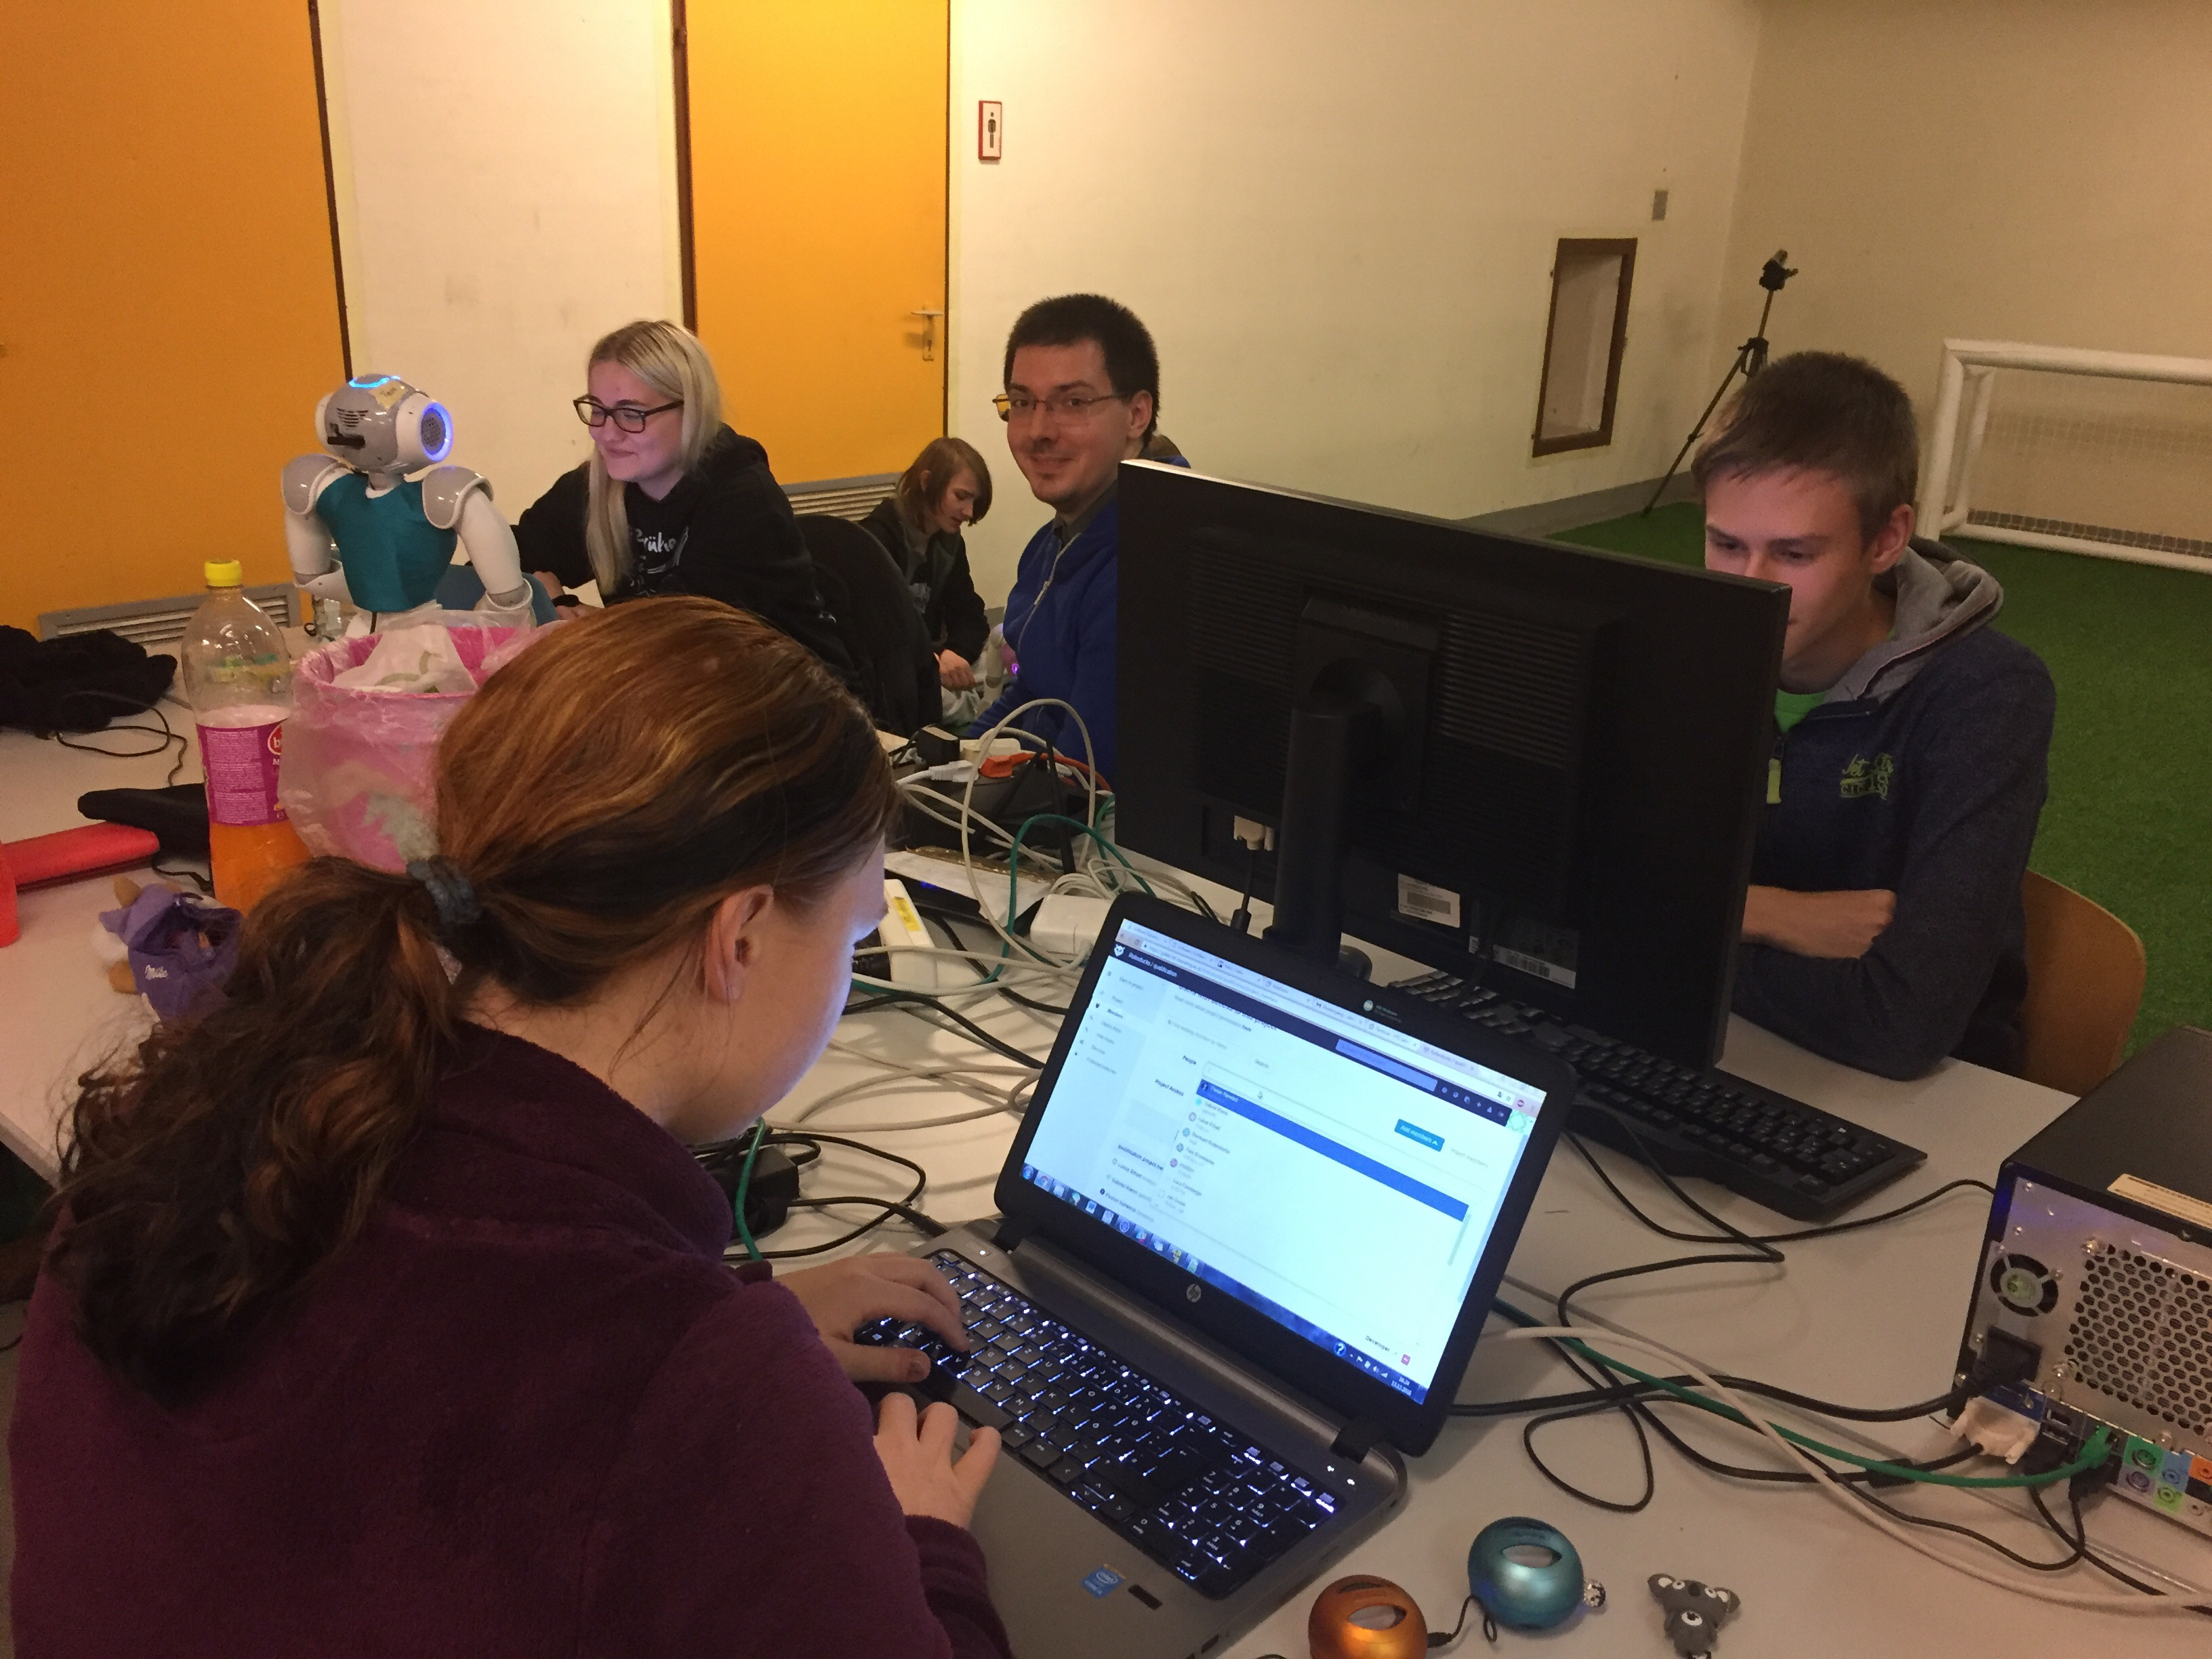
\includegraphics[scale=.063]{img/MotionTeam.jpg}
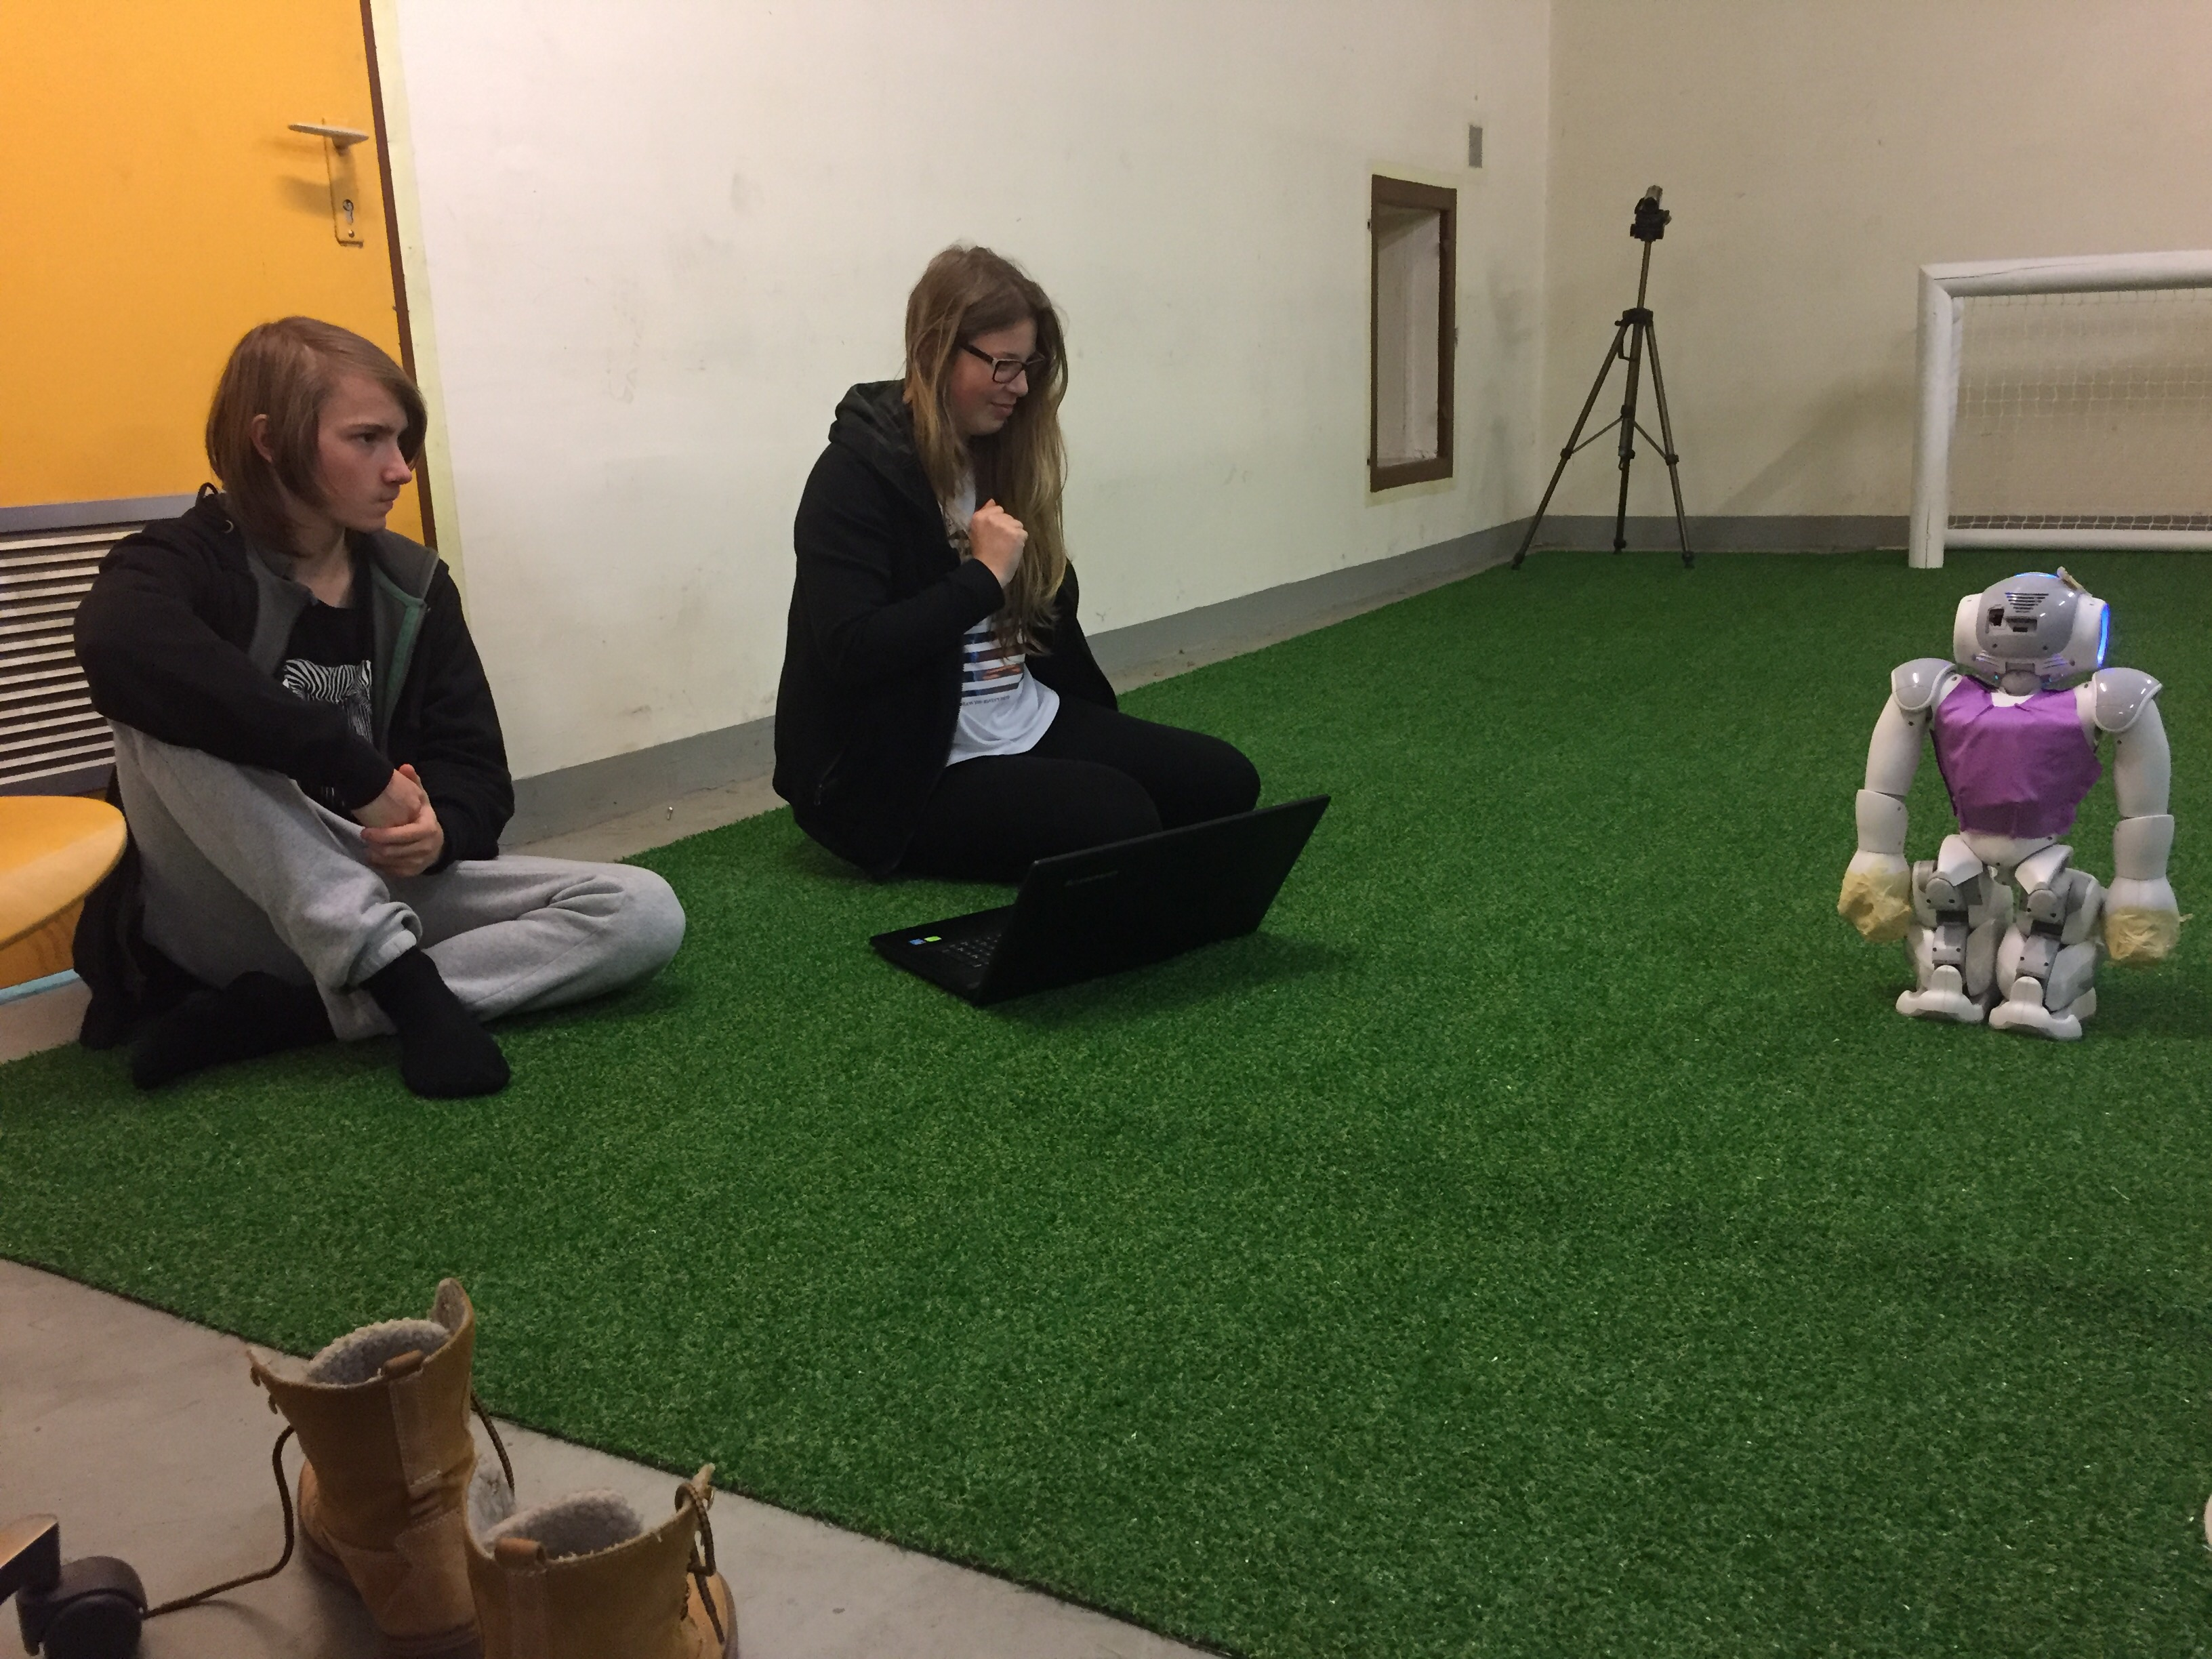
\includegraphics[scale=.063]{img/VisionTeam.jpg}
\end{center}
\caption{The Nao Team at its new home}\label{fig:motionteam}
\end{figure}

Besides informal working meetings the teams meet regularly every two weeks on Tuesday afternoons to align and bring the software together.

\section{Current State}\label{sec:state}
The 2017 SPL rule book brought a few changes, which are keeping the RoboDuck team pretty busy:

\begin{itemize}
	\item Switch field surface to 8 mm artificial turf (similar to what was used in the 2016 SPL Outdoor competition)
	\item Move towards more natural lighting
	\item Discontinuation of the Drop-in Player Competition
	\item Addition of a mixed teams competition on a larger field, where two teams combine to make a large (10 or 11) player team.  Entry into this competition will be limited due to time and space.
\end{itemize}

Currently we are working on the 8 mm artificial turf problem which has a tremendous impact on the complete motion part of our software. Even the successful teams of the RoboCup~2016 have severe difficulties to cope with this situation. Current attempts to introduce more sweeping leg movements caused high instabilities of the complete robot. In parallel to this we are continuously driving forward our vision software to detect and follow the ball. Here we are still not at the end but a good progress can be seen.

The Mills-Team which started only six weeks ago is currently on a good way to fix the vision part. The game field can be already recognized in a stable manner. In parallel we are now going into the motion area, where mastering the Nao Qi API is typically a longer lasting process for all newcomers in the Nao programming field. 
\section{Planned Activities for 2017}

\begin{itemize}
	\item {\em Tag der offenen Tür at the HTL Leonding (Jan 26 and 27, 2017):} As usual we will be here and present our latest software. We are currently working hard to be able to show an autonomous kick off and a goal kick of a Nao on the artificial turf as described above.
	
	\item {\em RoboCup German Open 2017, Magdeburg (May 5 to 7, 2017):} We plan to be in a playable mode by end of March, mid of April. From this time onwards we have to look for soccer competitions to get an idea of the quality of our work. The German Open would be a great opportunity here. We will have a closer look into this (especially in terms of budgeting), after we succeed to keep our planned development milestones.
	
	\item {\em 1. Krone E-Mobility Play Days, Spielberg (September 29 and 30, 2017):} Another possibility to proof our competitive ability. It would be a chance to play against the Nao Devils from the TU Leipzig and the Austrian Kangaroos from the TU Vienna and the University of Applied Sciences Technikum Wien.
	
	\item {\em Messe Jugend und Beruf (October 11 to 14, 2017):} Another fixed date where we traditionally take part in. Due to limited space at this site we will not present any soccer software but maybe we can show something new from our RoboMills team.
	
	\item {\em Increase Marketing Activities:} In cooperation with our colleagues from the department of media technique we want to set up a web site and a promotional video in order to make our activities better visible to a wider audience.
\end{itemize}

\section{Acknowledgements}
This project would not be possible without the kind support of several persons and organizations. We would like to express our gratitude to:

\begin{itemize}
	\item \emph{Absolventenverein der HTL Leonding (AbsLeo):} The AbsLeo accompanies this project since 2009. It budgeted the initial hardware which allowed us to get first experience with the Naos. Although it was clear that the whole journey will be a long one we could rely on their constant support. Again it was the AbsLeo which granted the budget to renew our hardware with two Naos during this fall. This enabled us to continue our ambitions towards participating the RoboCup World Championships.
	
	\item \emph{Management of the HTL Leonding:} Every project needs the great support from its embedding organization. All the smaller and larger organizational issues we are facing can be solved by means of the friendly support of our school. This is enabled by our head master and the two heads of departments. We are very happy to know that we can rely on them.
	
	\item \emph{Thomas Himmelbauer:} Despite his tough schedule as our school's IT manager he is a great technical supporter of our project. Without him our progress would have never been the one we have. His great expertise in the area of the C++ toolchain as well as his patience to figure out solutions concerning the NaoQi are really priceless.

	
	\item \emph{Alexander Hofmann (University of Applied Sciences Technikum Wien):} As the mastermind of the Austrian Kangaroos (who already took successfully part in several RoboCup competitions) we have a favourable partner in our area who stands on our side concerning lots of tips and advices to get part of the RoboCup community.
	
	\item \emph{Parents:} The support from our parents is a really great one. If it comes to pretty hands-on things like tailoring jerseys for our robots or getting a perfect construction for our goal we can heavily count on them. Thanks a lot for this.
\end{itemize}

\appendix
\section{The New Students Team Members}
The following table lists the newcomers sorted by classes: \\

\begin{tabular}{|l|l|l|l|l|}
\hline
	Class & Name 1 & Name 2 & Name 3 & Name 4 \\
	\hline
	2AHIF & Christian Bachl & Simon Danninger & Christoph Pfleger & Luis Noisternig \\
	\hline
	2BHIF & Erik Mayrhofer & Josef Gruber &&\\
	\hline
	2CHIF & Stefan Brandmair &&&\\
	\hline
	3AHIF & Severin Berger & Robin Gugl & Tobias Kneidinger &\\
	\hline
	3BHIF & Elias Schächel & Florian Harwöck & Gabriel Krenn & Lukas Erhart \\
	\hline
\end{tabular}

\end{document}  